\resetfigpath{intro}
\glsresetall

\chapter{Introduction}
\label{intro}

The medical imaging field has recently witnessed the revolution of \gls{ai}, a broad discipline that is part of computer science, whose aim is to conceptualize human ``intellectual'' tasks, and produce computer programs that can replicate them, thereby allowing to relieve human beings from tedious and repetitive tasks.
From classification to segmentation tasks, \gls{ai} already provides flexible and efficient tools that greatly facilitate the daily practice of clinicians.
In particular, large quantities of \gls{mri} brain scans are now efficiently and accurately processed by \gls{ai} systems that help clinicians in the diagnosis of pathologies \cite{sun19}.
Similarly, surgical instruments can be segmented automatically and accurately in real-time to allow laparoscopic interventions of the abdominal cavity by means of robotic technology, thereby decreasing the invasiveness of traditional methods \cite{davinci}.

Before diving into the underlying intricacies of these systems, we
first wish to give the reader some insights on the genesis of \gls{ai}.
In particular, we describe the two main paradigms that underlie common automated systems, namely the conventional programming and machine learning paradigms.
In a second section, we explain why one needs large amounts of annotated data to make modern \gls{ai} solutions practical, and how the medical imaging field, in particular, is hindered by this requirement.
Next, we emphasize how the present thesis aims at solving this issue.
Last, we give an overview of the organization of the present thesis.

\section{Conventional Programming VS. Machine Learning}
\Gls{ml}, a term that denote a sub-category of \gls{ai}, is grounded on the ``learning by example'' paradigm.
Whereas the conventional programming paradigm consists in explicitly formalizing and implementing complex tasks as a combination of simpler programmatic instructions,
\gls{ml} rather considers that a flexible system can learn such instructions automatically through repeated experiences.
While both paradigms are in practice complementary, the general trend in many research domains such as computer vision, medical image analysis, computer-assisted intervention in medical applications, shows an increasing shift toward the predictive paradigm, on which \gls{ml} approaches are based.
We wish to give the reader some insights on the main differences between these two paradigms.
We first give some generalities, and show, through a concrete example, how the \gls{ml} paradigm can overcome the limitations of conventional programming.

The term \gls{ml} can be dated back to 1959, where it appears in the seminal work of Arthur Samuel: \textit{Some studies in machine learning using the game of checkers} \cite{samuel59}.
The author defines \gls{ml} as \textit{a field of study that gives computers the ability to learn without being explictly programmed}.
The pretext goal of the latter work is to produce a computer program that can play the game of checkers with reasonable skill, i.e. be a challenging opponent to a human player, while overcoming the limitations of the conventional programming paradigm.

First, the author emphasizes that this game, however simple it may seem when compared to chess, allows a very large number of possible different games: around $10^{40}$.

Before delving into the \gls{ml} approach, let us first describe how a typical conventional approach would work, so as to emphasize the inherent challenges that it would have to overcome.
First, as the number of situations, i.e. the possible configurations of the checker-board, is very large, the programmer would first need to gather and analyze a representative set of possible checker-board configurations, and devise a fixed set of logical rules so as to determine, in each situation, the move that would guarantee a win.
In particular, a skilled player, which the machine must mimic, combines different intermediate goals so as to reach the final goal of winning the game, e.g. capturing many opponent's pieces without losing one's own pieces, and improving the overall positioning of pieces.
Furthermore, assuming the above sub-goals can be programmatically combined in a coherent and flexible manner, each one of them would require a logical reasoning that would span several turns, both backward and forward.
In this particular example of the game of checkers, one sees that devising such set of rules is tedious and error-prone, as the programmer is at risk of missing or misspecifying important combinations.

A typical \gls{ml} approach would rather consider a flexible model that includes a large and redundant set of parameters, which need to be combined through mathematical operations to output an optimal decision.
Furthermore, such model is designed to integrate elementary knowledge related to the rules of the game.
Importantly, the programmer does not specify in advance, as was the case in the conventional programming paradigm, which operations need to be applied to which parameter, and what importance (also called weights) to give to each one of them.
The key component of the \gls{ml} approach is then to devise a training procedure, which consists in optimizing these parameters by minimizing an error, taken as a discrepancy measure between the system's output and the desired output.

In particular, the model is given, throughout the training procedure, inputs that consist in a numerical representation of the checker-board, possibly with a history of previous checker-board configuration.
At the beginning of the training procedure, the model is totally ignorant of the complex decision making process, and will typically produce a poor move.
The \textit{goodness} of this move will be assessed using a reference ``good'' move, which an expert checker player has generated by looking at the same checker-board.
In order to exploit this knowledge, the programmer must therefore define in advance a quantitative measure of goodness, usually called \textit{error}.
Next, an update scheme allows to update the numerous parameters of the model so as to minimize the error.
Simply put, if the error is large, we would like to encourage the model to produce a drastically different move when facing a similar checker-board configuration.
Conversely, when the move is adequate to the expected move, the model must give a high priority to the latter decision.
Intuitively, one sees that a single experience of this kind does not allow to fully explore the strategic depth of the game.
One therefore needs to generate a large number of such experiences so as to make the model capable of competing against creative and competent human opponents.
The above paradigm, which stands at the root of \gls{ml} is called ``learning by example'', and conveys the idea that machines are able to learn to perform complex tasks \textit{without being explictly programmed to do so}, through repeated experiences.

In practice, however, conventional and \gls{ml} paradigms are often used complementarily.
For example, in the present scenario, an early-stage instance could allow to select among different game strategies selected by a pre-defined algorithm, e.g. ``aggressively give-away pieces'', ``play conservative'', and let the trained module select which move to perform within it.

We now wish to emphasize the fact that \gls{ml} approaches, which in principle allows to solve more and more complex tasks, comes with its own limitations, namely that the considered model must be able to explore an increasingly large amount of situations, while its decisions must be compared to reference outputs.
In the \gls{ml} terminology, we call such input data coupled with its reference output a \textit{training sample}.
In practice, producing these reference outputs (called \textit{annotations} or \textit{labels}) often requires human interventions, in which human experts
are shown a serie of inputs, and must provide the ``optimal'' output.

From these considerations, we pull out the following rule-of-thumb.

\textbf{\textit{As the complexity of the task increases, \gls{ml}-based solutions require an increasing amount of annotated training samples to be effective.}}

We now elaborate on the fact that the latter requirement constitutes a bottleneck in the deployment of modern \gls{ml} methods, as many fields of applications, and in particular medical imaging applications, require intensive contributions of trained experts.

\section{On the growing importance of large quantities of annotated data}
In their most primitive form, \gls{ml} methods consider that the model to train takes as input a pre-defined numerical representation of the ``situations'', which we now prefer to call \textit{features}.
In the previous example of checkers, the feature encoding is a set of numbers corresponding to the position on the check-board and the occupancy of that position.

Extracting such set of features was originally a preliminary ad-hoc step, while the design and training of the late-stage \gls{ml} model formed another step.
Engineers had to devise for the task at hand a feature extraction method, in such a way that this encoding embodies a wide spectrum of situations in a dense and sufficiently rich form.
The latter task was in itself tedious and cumbersome, as it presupposes that the engineer understands the full range of characteristics of these situations, which characteristics are relevant, and how to quantify them.

More recently, thanks to the technical progress in computing hardware, \gls{dl}, a class of models that elaborate on \gls{nn}, allowed to overcome this limitation.
In essence, \gls{dl} models allow one to train both the feature extraction instance and the predictive instance in a joint manner, i.e. through the optimization of both instances through an update scheme devised from a single objective.
This has brought spectacular improvements in performance over traditional methods, making \gls{dl} the de-facto standard in many fields of application, e.g. classification and segmentation of images.
As will be further developed in a next chapter, \gls{dl} models are composed of a concatenation of layers that each perform simple mathematical operations, such as matrix multiplication or convolutions.
The power, flexibility, and hence impressive performance boost of \gls{dl} models, namely comes from the fact that stacking many layers allows to produce rich and abstract features, while the same principle allows the predictive instance to model complex interactions between the components of feature vectors.

As showcase application, let us mention the ImageNet Large Scale Visual Recognition Challenge \cite{ILSVRC15}, which consists in classifying natural images into semantic categories such as ``balloon'', ``dog'', etc..
The inputs are taken as the images themselves, i.e. a square-grid where each cell represent a pixel that encodes $3$ numerical values: one for each color channel.
The training dataset contains $150'000$ images, classified into $1000$ categories.
As of today, state-of-the-art solution leverage \gls{dl}-based models.
In particular, Deep Convolutional Neural Network can classify unseen images with an accuracy of $88.6\%$ \cite{tan19}, a performance on par, if not superior, with human skills.
The full model contains a feature extraction module, which extracts salient characteristics of the image such as texture, colors, and shapes.
At its output lies a classification module, which is responsible to combine these features through cascaded mathematical operations.
In order to get and idea of the complexity of the task, think about recognizing a dog in an image taken at random from the internet, and try to evaluate the huge variety of situations in which such object can appear, e.g. field of view of the photographer, position of the dog, lightning condition, breed of the dog, clutter in the background.
Next, multiply this already daunting task to a thousand kind of objects, and you will easily understand why the latter state-of-the-art model accounts for over $70$ million parameters.
Let us emphasize that, in this scenario where natural images must be classified, the tedious task of annotating training images has been performed by many individuals in parallel, an approach called \textit{crowd-sourcing}.

Another example, closer in nature to the present thesis, is the Brain Tumor Segmentation (BraTS) Challenge \cite{menze15}, which consists in segmenting brain tumors from \gls{mri} scans, where the model needs to output for each pixel of a given slice a prediction that will help a clinician in his/her diagnosis.
State-of-the-art \gls{dl} models typically account for $\sim 50$ million parameters \cite{chen19}, which are trained using $450$ annotated scans, each containing $\sim 70$ slices (see Fig. \ref{fig:brats}).
A first requirement for the training of such model, is that each pixel of each slice has to be annotated several times to account for disagreements between medical experts.
Second, tumors are often composed of several distinct regions, e.g. necrotic and non-enhancing tumor, peritumoral edema, and enhancing tumor \cite{akil20}.
All in all, annotating a full MRI scan is estimated to take between 3 and 5 hours of work \cite{kaus01}.


\begin{figure}[!htpb]
  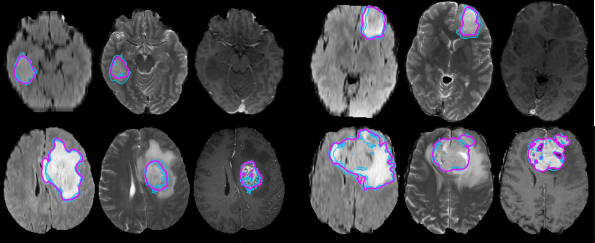
\includegraphics[width=0.99\textwidth]{brats.png}
  \caption{Examples from the BRATS dataset. Annotation of individual experts are in blue, consensus segmentations are in pink. Taken from \cite{menze15}}
  \label{fig:brats}
\end{figure}

As a last example, let us mention the Robotic Instrument Segmentation Challenge \cite{allan19}, where a variety of surgical instruments, part of a minimally invasive surgical robot, must be detected.
In particular, the provided set consists of $10$ videos, each containing around $300$ frames.
Also, each frame can contain several instruments, while each instrument contains several parts that must be annotated separately.
An example of the provided images and annotations is shown in Fig. \ref{fig:intro_endovis}.
The annotation time is estimated to $1$ minute per image per instrument.

\begin{figure}[t!]
    \centering
    \begin{subfigure}[b]{0.5\textwidth}
        \centering
        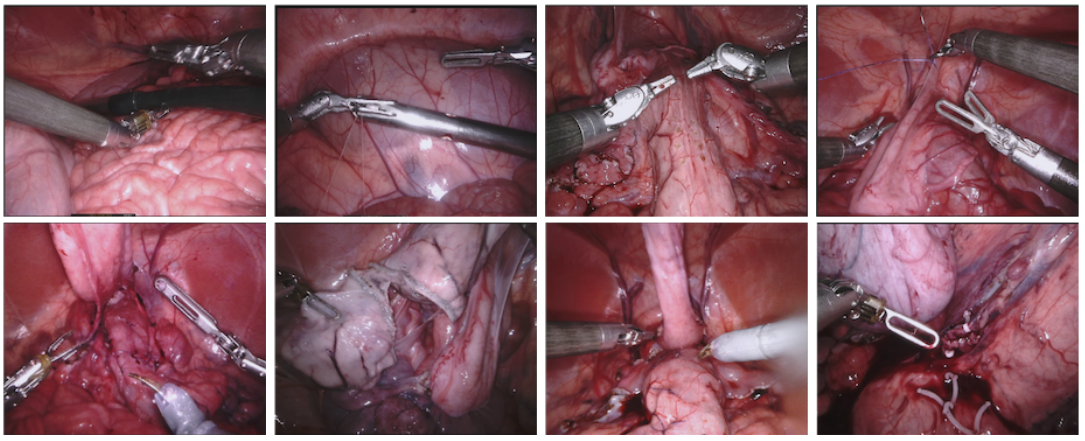
\includegraphics[height=3cm]{endovis_trainset}
        \caption{Examples frames from the training set.}
    \end{subfigure}%
    \begin{subfigure}[b]{0.5\textwidth}
        \centering
        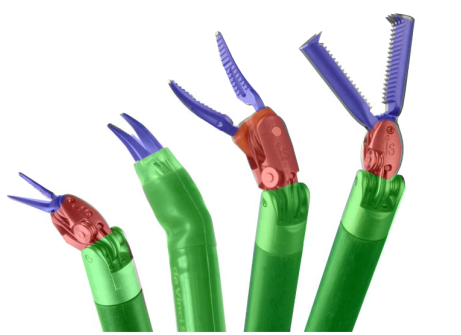
\includegraphics[height=3.5cm]{endovis_gt}
        \caption{Examples of pixel-wise semantic labels on different instruments}
    \end{subfigure}
    \caption{Examples from the EndoVision surgical instrument segmentation challenge. Taken from \cite{allan19}.}
    \label{fig:intro_endovis}
\end{figure}

\section{Problem definition and thesis statement}

Comparing the above scenarios, we emphasize that applying state-of-the-art \gls{dl} methods to the segmentation of medical images poses additional practical difficulties with respect.
In particular, the annotation task requires a medical expertise.
Second, assuming such experts are available and willing to participate to this task, their daily obligations usually imposes a limited time budget.
Third, the task itself is considered tedious and repetitive.
These three factors alone largely explain why the field of medical imaging tends to not benefit from the latest \gls{dl} technologies used in more generic applications \cite{orting19}.

\textbf{Problem definition}
The present thesis addresses the bottleneck of scarcity of annotated medical images by proposing a fast and intuitive annotation protocol, along with appropriate segmentation methods that allow to generate accurate segmentation of objects of interest on a wide variety of medical imaging modalities.

\textbf{Thesis statement}
Generating pixel-wise annotations of medical sequences over a wide range of modalities is greatly facilitated by means of a novel fast and intuitive protocol that relies on sparse point-wise cues, aided by a segmentation framework that relies on \gls{dl} and multi-object tracking.

\section{Organization and Contribution of this Thesis}
The organization of this thesis is now summarized per chapter:

\textbf{Chapter 2} gives an overview of the broad literature related to the present thesis.
In particular, we first give a state-of-the-art of computer vision methods related to segmentation of images and volumes using sparse annotations.
Next, we review several categories of \gls{ml} methods related to the present scenario, namely \gls{ssl}, \gls{pu}, and \gls{da}.
Last, we add some essential theoretical elements that intervene in the solutions proposed in the present thesis.

\textbf{Chapter 3} gives a detailed description of our fast point-wise annotation protocol.
In particular, the requirements of our annotation protocol are given in detail and justified.
Next, we describe our software solutions, namely a cross-platform and multi-device annotation software, and a web platform with a frontend that allows users to upload annotations, while a backend runs our segmentations algorithms.
We then describe the medical datasets that were used for the evaluation of the proposed segmentation methods, and emphasize how they cover a wide spectrum of real-world use-cases.

\textbf{Chapter 4} contains our first segmentation method that relies on the Expected Exponential loss, optimized using a gradient boosting classifier. The probabilities of unlabeled samples are estimated using label propagation.

\textbf{Chapter 5} gives a thorough study of feature extraction methods, which form an important component of the method presented in the next chapter.
In particular, we first develop an evaluation framework based on a \gls{rf} classifier that operates on superpixels.
As baselines, we implement traditional feature extraction methods, such as \gls{bovw}.
Another baseline considers unsupervised deep feature extraction, where we use a \gls{cnn} trained to classify natural images.
We then implement various methods based on \gls{dl} that integrate motion priors, as well as priors derived from the user-provided point annotations.
Through extensive experiments, we demonstrate the superiority of the \gls{ae} configuration aided by spatial priors.

\textbf{Chapter 6} presents an innovative framework based on multi-object tracking.
Concretely, we formulate our segmentation problem as a maximum a-posteriori problem, where the random variable to optimize is the objectness of superpixels.
Using deep features extracted with the best method of the previous chapter, we train an ensemble of decision trees using a sampling method applicable to the \gls{pu} setup.
Next, simple gaussian kernels provide pairwise similarity measures.
These two models allow to define likelihoods of selecting a superpixel given the user's annotations, and transiting from one frame to the next.
Using the network flow paradigm, we then build a graph that connects superpixels according to spatio-temporal relations.
This chapter covers the content of our first journal article \cite{lejeune18}.

\textbf{Chapter 7} investigates on using a self-supervised clustering method to improve on the foreground prediction and pairwise similarity models defined in the previous chapter.
In particular, our original ambition was to use the self-supervised embedded clustering paradigm to generate pairwise similarity labels.
Our next step would then consist in training a pairwise similarity module, using the above labels.
Even though this approach did not show substantial improvements in performance, we choose to mention it here as a negative result.

\textbf{Chapter 8} continues on the same line as the previous chapter by improving on the foreground prediction model.
Instead of using two components, where the first generates deep features, while the second estimates foreground probabilities, we aim at combining the two in an end-to-end fashion.
We leverage a loss function applicable to the \gls{pu} scenario, where the foreground probabilities are inferred by a deep network configured as a predictor.
As the latter loss function requires accurate class priors to render its full potential, we further devise a strategy to estimate the latter in a self-supervised manner.
In particular, our approach consists in setting an initial upper-bound constant value (possibly misspecified) on the prior, and gradually decrease the latter using as evidence the output of the deep network.
Our algorithm relies on the recursive bayesian estimation paradigm.
This chapter covers the content of our second journal article, currently in preparation.

\textbf{Chapter 9} gives a summary of our contributions, provides general discussions on the improvements and limitations of our solutions, and concludes by giving an outline on future works.

%%% Local Variables:
%%% mode: latex
%%% TeX-master: "../../main"
%%% End:
